\documentclass[11pt,a4paper]{article}

\usepackage[margin=2.2cm]{geometry}
\usepackage[T1]{fontenc}
\usepackage{lmodern}
\usepackage{microtype}
\usepackage{graphicx}
\usepackage{booktabs}
\usepackage{tabularx}
\usepackage{longtable}
\usepackage{array}
\usepackage{pdflscape}
\usepackage[table]{xcolor}
\usepackage{enumitem}
\usepackage{caption}
\usepackage{float}
\usepackage{subcaption}
\usepackage{listings}
\usepackage{tikz}
\usetikzlibrary{positioning,fit,arrows.meta,backgrounds}
\usepackage[htt]{hyphenat}   % allow line breaks inside long monospace identifiers
\usepackage[hidelinks]{hyperref}

\definecolor{jade}{HTML}{0B3D30}
\definecolor{jadelight}{HTML}{E1F0E8}
\definecolor{coral}{HTML}{B8412B}
\definecolor{corallight}{HTML}{FBE7E2}
\definecolor{codebg}{HTML}{F3F5F2}

\captionsetup{font=small,labelfont=bf}
\setlist{itemsep=2pt,topsep=4pt}
\setlength{\parskip}{4pt}
\setlength{\emergencystretch}{3em}
\renewcommand{\arraystretch}{1.25}
\newcolumntype{Y}{>{\raggedright\arraybackslash}X}
\newcolumntype{P}[1]{>{\raggedright\arraybackslash}p{#1}}

\lstset{basicstyle=\ttfamily\footnotesize, backgroundcolor=\color{codebg}, frame=single, rulecolor=\color{black!15},
        breaklines=true, columns=fullflexible, keepspaces=true, xleftmargin=4pt, xrightmargin=4pt, aboveskip=6pt}

\newcommand{\W}[1]{\textbf{#1}}
\newcommand{\numtests}{39}
\newcommand{\code}[1]{\texttt{#1}}

\begin{document}

% ------------------------------------------------------------------ title
\begin{titlepage}
\centering
\vspace*{2.5cm}
{\Large CY-5004 Secure Software Design\par}
\vspace{0.4cm}
{\large National University of Computer and Emerging Sciences, Islamabad\par}
\vspace{2cm}
{\Huge\bfseries SecureWallet\par}
\vspace{0.4cm}
{\Large Assignment 1: Mini Secure Fintech Wallet\par}
\vspace{2cm}
\begin{tabular}{ll}
\toprule
Instructor & Muhammad Asim \\
Group members & Israr Ahmed (26I-7722) \\
 & Burhan Ud Din (26I-7711) \\
Submission date & 2 October 2026 \\
\bottomrule
\end{tabular}
\vfill
{\small Source code: \code{A1/} (Docker Compose project). Run instructions: \code{README.md}.\par}
\end{titlepage}

\tableofcontents
\newpage

% ------------------------------------------------------------------ 1
\section{System overview}

SecureWallet is a small digital wallet. Registered customers hold a balance in Pakistani rupees and send it instantly to any other customer by username. It implements all six operations required by the brief (Table~\ref{tab:ops}) and protects them with thirteen security controls. Each control answers one weakness identified in Section~\ref{sec:weak}, has a before/after demonstration, and is covered by an automated test. All \numtests{} tests pass.

\begin{table}[H]
\centering\small
\caption{Required operations and how SecureWallet provides them.}
\label{tab:ops}
\begin{tabularx}{\textwidth}{P{4.2cm}Y}
\toprule
Operation (brief \S1) & Implementation \\
\midrule
Create / use an account & Sign-up with full name, username and password. Each account gets exactly one wallet. Demo accounts are seeded: \code{ali}, \code{sara}, \code{bilal}, \code{hina} (customers) and \code{auditor}. \\
Log in & Username and password. The session ends after 5 minutes without activity. Transfers above a risk threshold also need a passkey (fingerprint, face or device PIN). \\
View balance & Balance card on the home screen, refreshed after every transfer. \\
Transfer funds & Send flow, laid out as a cheque: payee $\rightarrow$ amount (also written out in words) and memo $\rightarrow$ review, signed with the 6-digit transaction PIN $\rightarrow$ send. Sender is debited, receiver credited, one transaction recorded. \\
View transactions & Statement page: month sections with brought/carried-forward lines, sender, receiver, amount, date/time, status (completed or failed) and a running balance, with search and filters. \\
Log out & Sign out on this device, or on all devices from the Security page. \\
\bottomrule
\end{tabularx}
\end{table}

\paragraph{Technology.} A React 18 single-page application is served by nginx. It talks to a FastAPI (Python 3.12) backend, which stores data in PostgreSQL 16. The three services run with Docker Compose. Money is stored as whole \emph{paisa} (1 rupee = 100 paisa) in 64-bit integers, so no floating-point rounding can occur anywhere in a money path.

\paragraph{Interface.} The interface is laid out as a bank passbook: the home page is the account page and ledger with a running balance on every line, sending money is writing a cheque signed with the transaction PIN, and the receipt is its counterfoil (Figure~\ref{fig:app}). Amounts are also written out in words in the Pakistani lakh/crore system, as on a real cheque, which helps a user notice a mistyped amount.

\paragraph{Roles.} Customers hold and send money. A separate \emph{auditor} role can read the audit log and run a ledger reconciliation but cannot move money.

\paragraph{Presenter mode.} For the live demonstration, a hidden presenter mode (Ctrl+Shift+D) adds two tools:
\begin{itemize}
\item a \emph{security trace} panel showing every security check the server ran for each request, with real values;
\item a \emph{security lab} that switches each control off and on for the before/after tests in Section~\ref{sec:tests}.
\end{itemize}
Both exist only when the server runs with \code{DEMO\_MODE=true}. With the default \code{false}, the endpoints are not mounted at all.

\begin{figure}[H]
\centering
\begin{subfigure}{0.49\textwidth}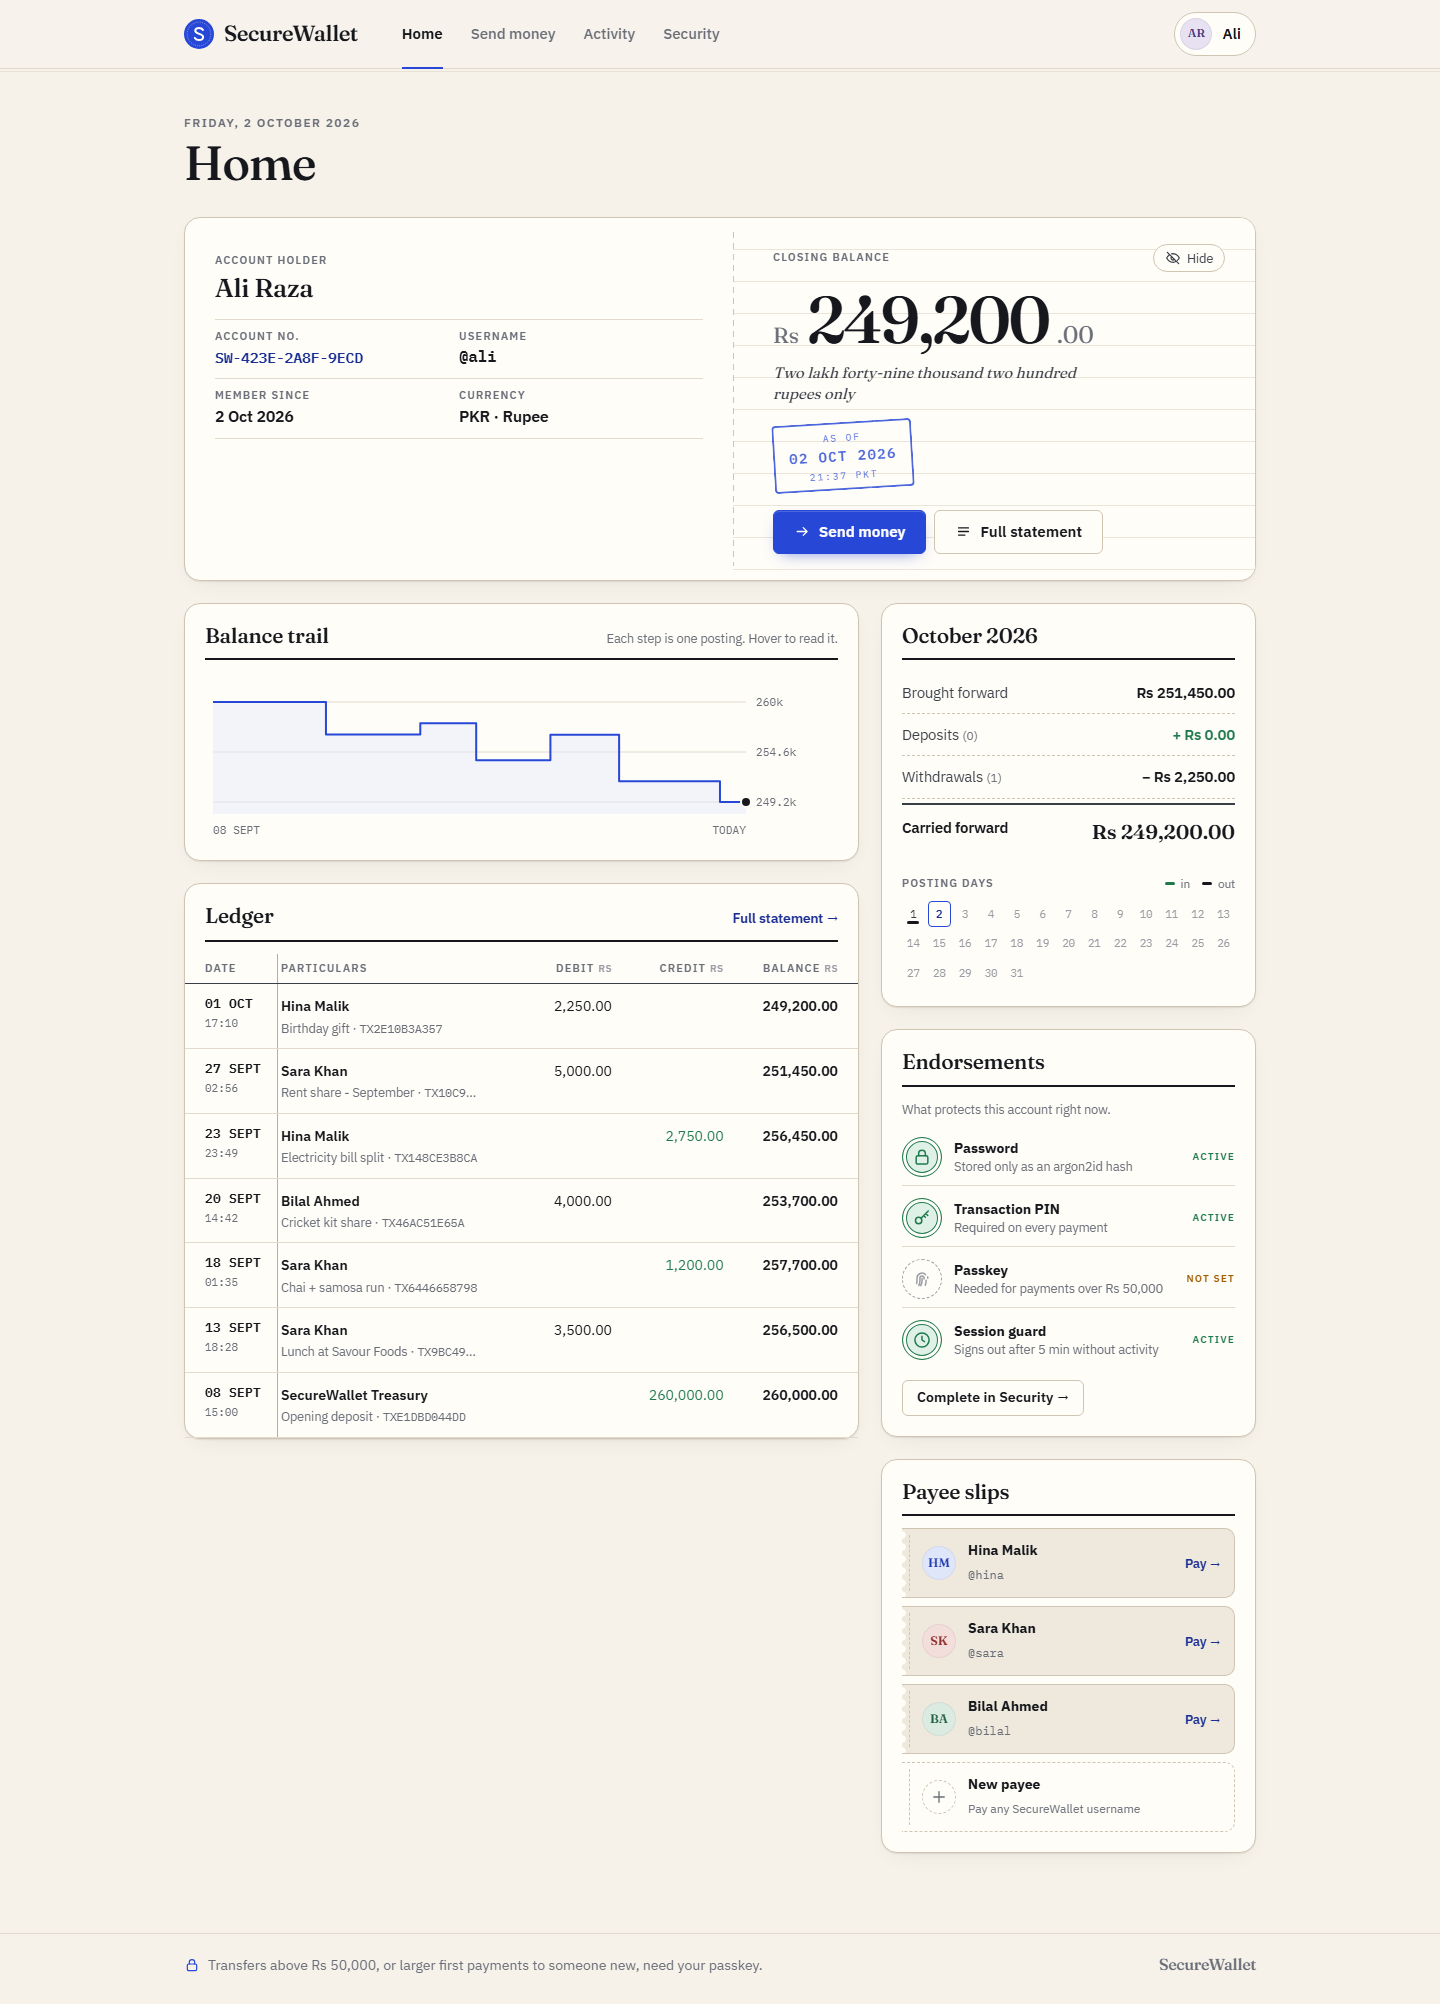
\includegraphics[width=\linewidth]{figures/v2-home.png}\caption{Home: account page, balance trail, ledger with running balance, month reconciliation and security endorsements.}\end{subfigure}\hfill
\begin{subfigure}{0.49\textwidth}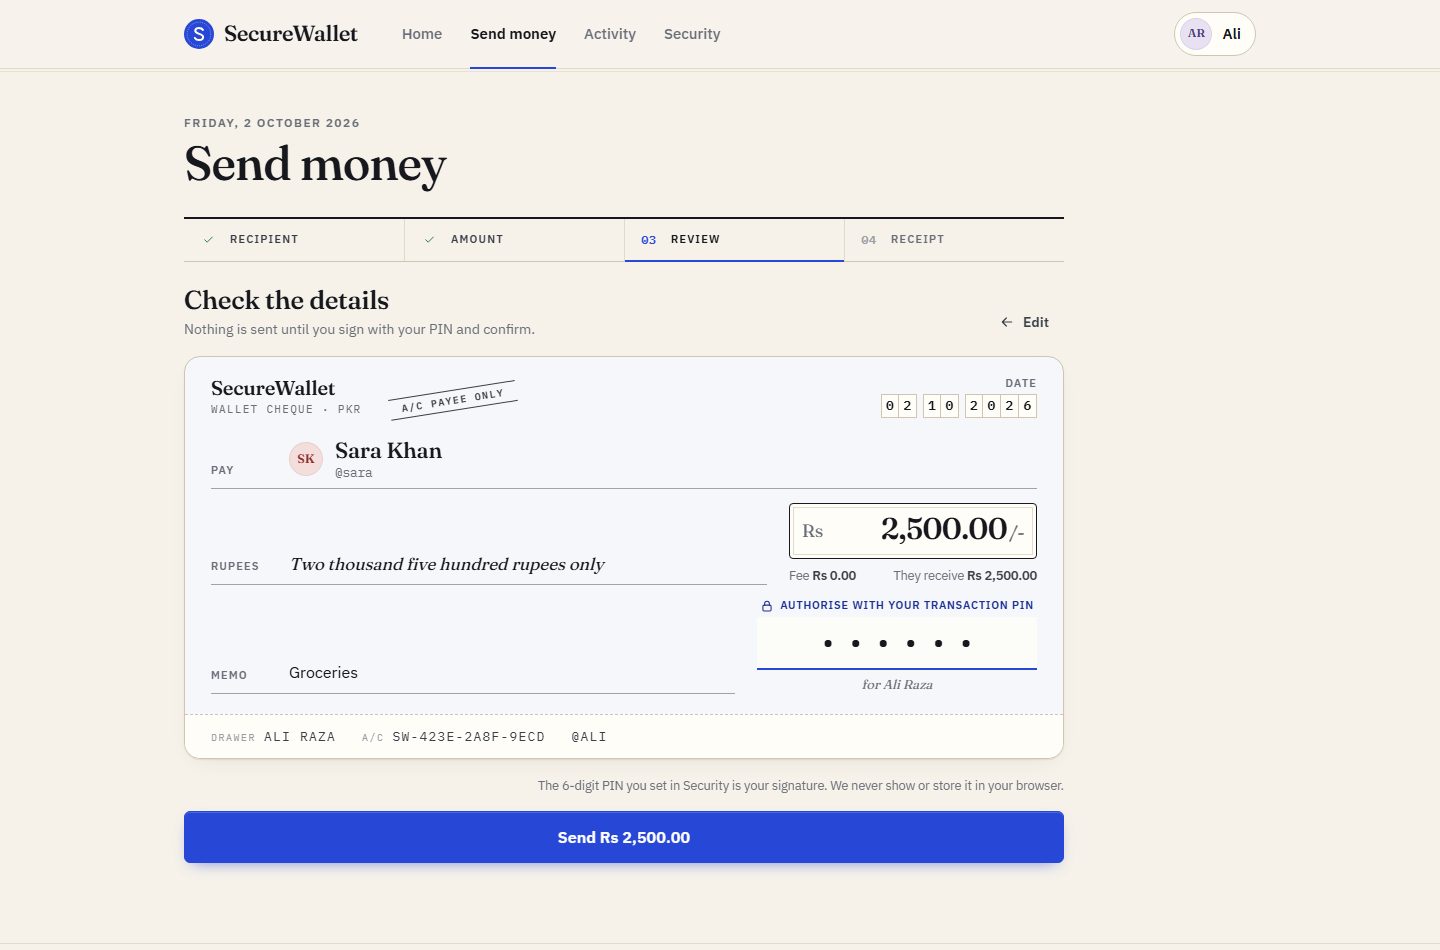
\includegraphics[width=\linewidth]{figures/v2-send-cheque.png}\caption{Send money: the cheque, amount in words, signed with the transaction PIN.}\end{subfigure}

\vspace{6pt}
\begin{subfigure}{0.49\textwidth}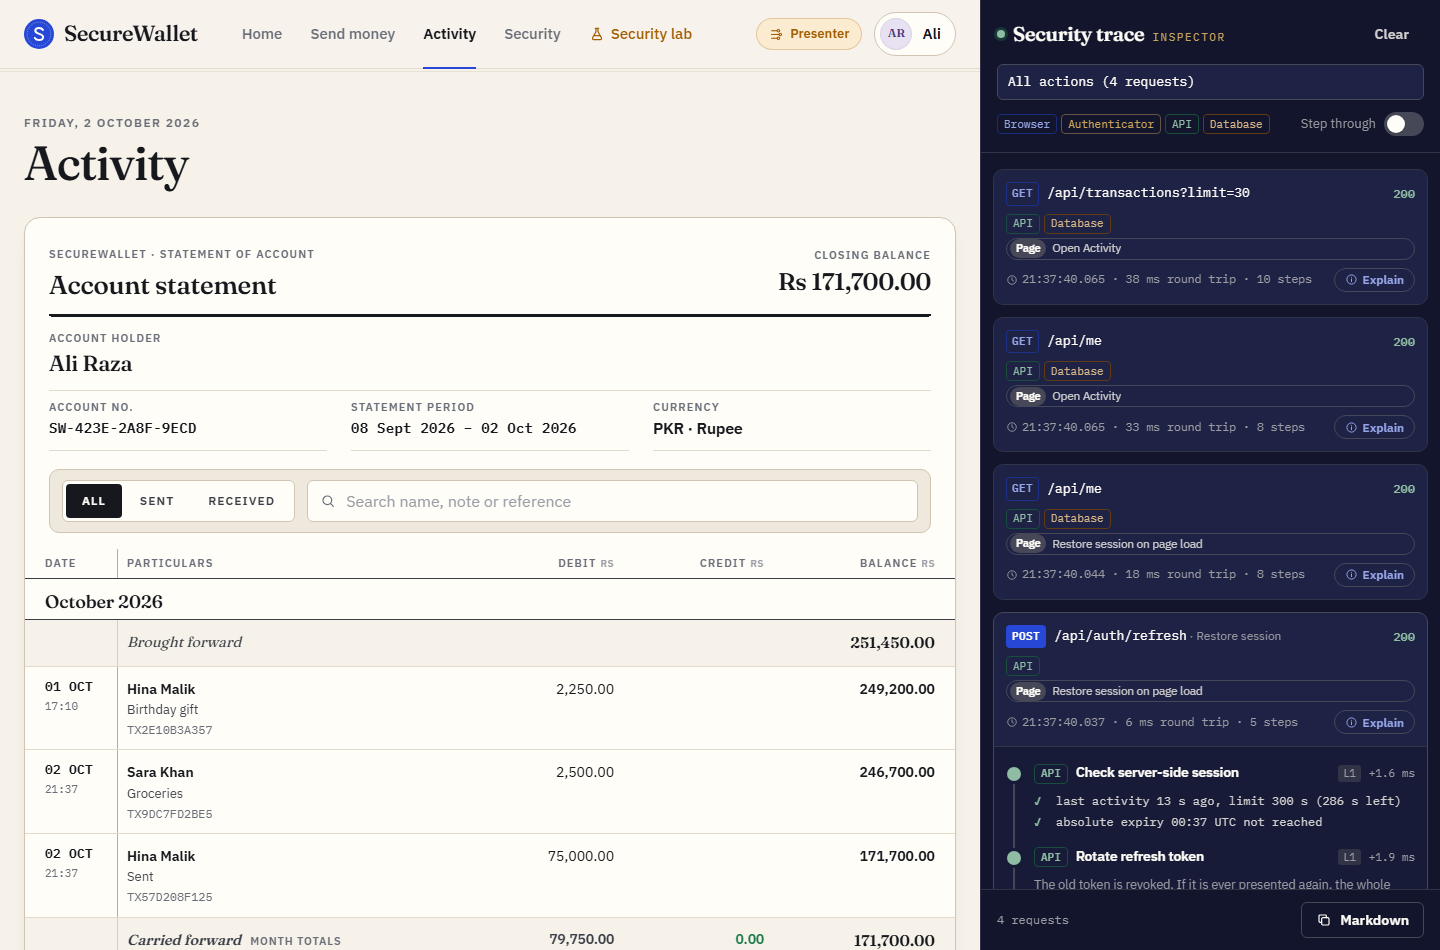
\includegraphics[width=\linewidth]{figures/v2-activity.png}\caption{Statement with brought/carried-forward lines and running balance.}\end{subfigure}\hfill
\begin{subfigure}{0.49\textwidth}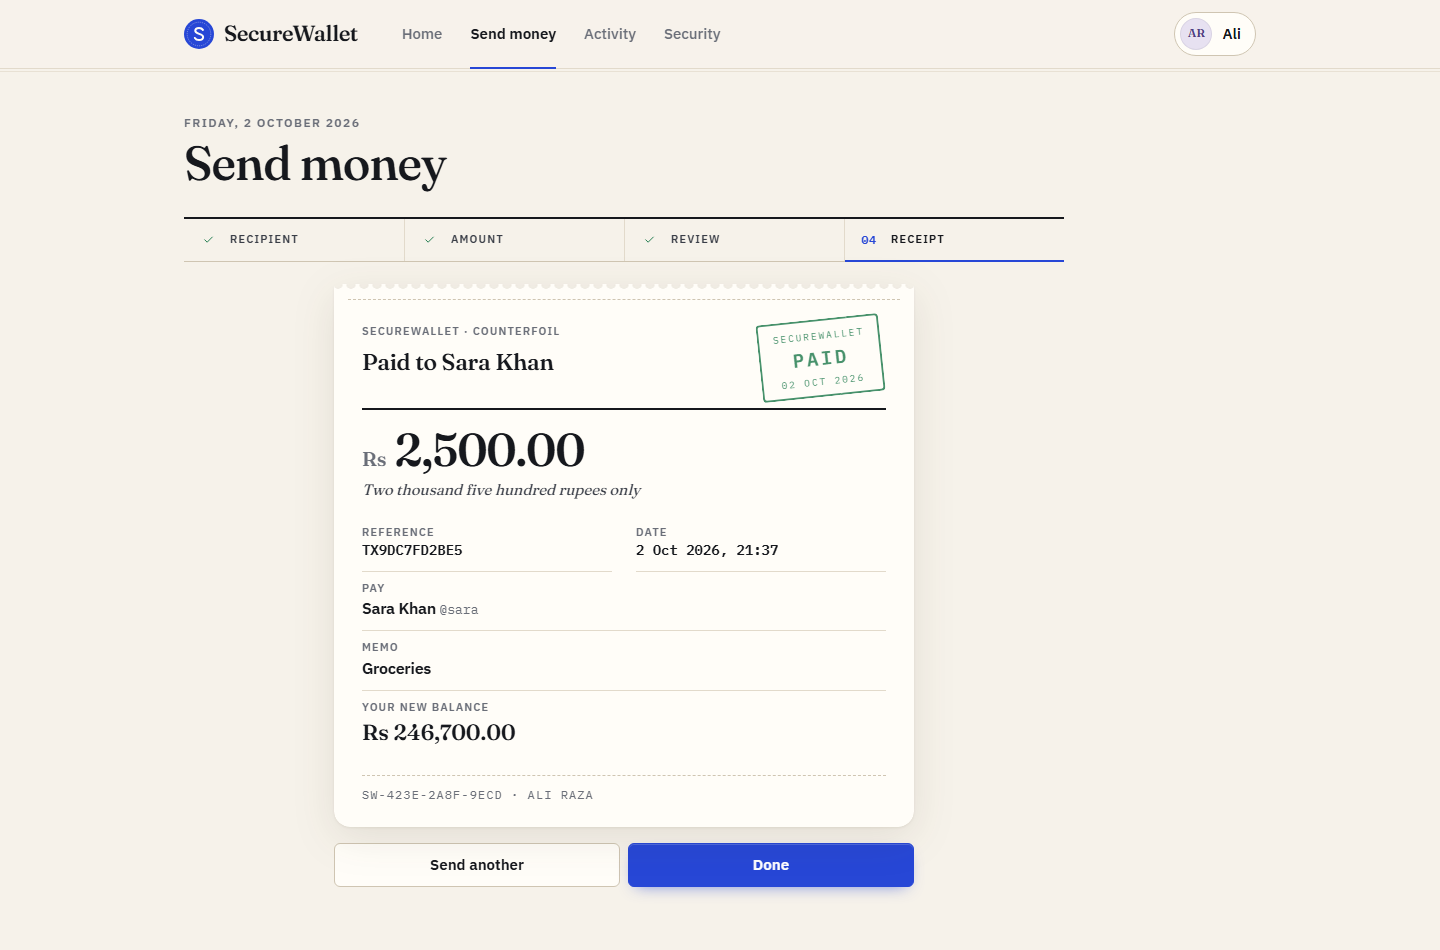
\includegraphics[width=\linewidth]{figures/v2-send-counterfoil.png}\caption{Counterfoil after a completed transfer, stamped PAID.}\end{subfigure}
\caption{The customer-facing application.}
\label{fig:app}
\end{figure}

% ------------------------------------------------------------------ 2
\section{Architecture}
\label{sec:arch}

Figure~\ref{fig:arch} shows the four components, the two Docker networks, and where each security control is enforced. The database has no published port and sits on an internal network with no route to the internet. Only the API can reach it. The API connects as a restricted database role, so the database itself enforces ownership and least privilege, even if the API code has a bug.

\begin{figure}[H]
\centering
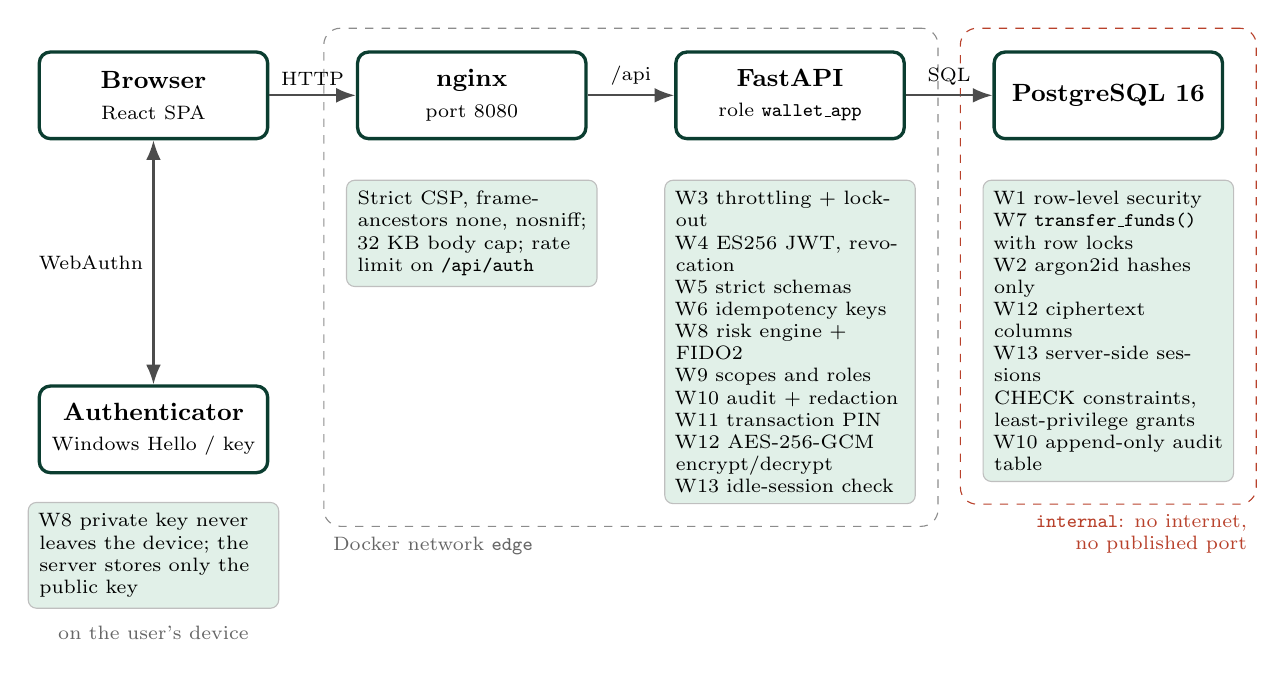
\begin{tikzpicture}[
  comp/.style={draw=jade, very thick, rounded corners=4pt, fill=white, minimum width=2.9cm, minimum height=1.1cm, align=center, font=\small\bfseries},
  ctrl/.style={draw=black!25, rounded corners=3pt, fill=jadelight, align=left, font=\scriptsize, text width=2.9cm, inner sep=4pt},
  net/.style={draw=black!45, dashed, rounded corners=6pt, inner sep=8pt},
  arr/.style={-{Latex[length=2.5mm]}, thick, draw=black!70},
  node distance=1.1cm and 1.1cm]

\node[comp] (browser) {Browser\\\normalfont\scriptsize React SPA};
\node[comp, right=of browser] (nginx) {nginx\\\normalfont\scriptsize port 8080};
\node[comp, right=of nginx] (api) {FastAPI\\\normalfont\scriptsize role \code{wallet\_app}};
\node[comp, right=of api] (db) {PostgreSQL 16};

\draw[arr] (browser) -- node[above, font=\scriptsize]{HTTP} (nginx);
\draw[arr] (nginx) -- node[above, font=\scriptsize]{/api} (api);
\draw[arr] (api) -- node[above, font=\scriptsize]{SQL} (db);

\node[ctrl, below=0.5cm of nginx] (c-nginx) {Strict CSP, frame-ancestors none, nosniff; 32 KB body cap; rate limit on \code{/api/auth}};
\node[ctrl, below=0.5cm of api] (c-api) {W3 throttling + lockout\\W4 ES256 JWT, revocation\\W5 strict schemas\\W6 idempotency keys\\W8 risk engine + FIDO2\\W9 scopes and roles\\W10 audit + redaction\\W11 transaction PIN\\W12 AES-256-GCM encrypt/decrypt\\W13 idle-session check};
\node[ctrl, below=0.5cm of db] (c-db) {W1 row-level security\\W7 \code{transfer\_funds()} with row locks\\W2 argon2id hashes only\\W12 ciphertext columns\\W13 server-side sessions\\CHECK constraints, least-privilege grants\\W10 append-only audit table};

\node[comp, below=3.1cm of browser] (auth) {Authenticator\\\normalfont\scriptsize Windows Hello / key};
\draw[arr, {Latex[length=2.5mm]}-{Latex[length=2.5mm]}] (browser) -- node[left, font=\scriptsize, align=right]{WebAuthn} (auth);
\node[ctrl, below=0.35cm of auth] (c-auth) {W8 private key never leaves the device; the server stores only the public key};

\begin{scope}[on background layer]
\node[net, fit=(nginx)(api)(c-nginx)(c-api)] (edge) {};
\node[net, draw=coral, fit=(db)(c-db)] (internal) {};
\end{scope}
\node[font=\scriptsize, anchor=north west, text=black!60] at (edge.south west) {Docker network \code{edge}};
\node[font=\scriptsize, anchor=north east, text=coral, align=right] at (internal.south east) {\code{internal}: no internet,\\no published port};
\node[font=\scriptsize, anchor=north, text=black!60] at ([yshift=-0.1cm]c-auth.south) {on the user's device};
\end{tikzpicture}
\caption{SecureWallet architecture and where each control (W1--W13) is enforced.}
\label{fig:arch}
\end{figure}

The controls follow the layered defence model from Lecture 2:

\begin{table}[H]
\centering\small
\caption{Controls by defence-in-depth layer (Lecture 2).}
\begin{tabularx}{\textwidth}{P{3.4cm}P{3.6cm}Y}
\toprule
Layer & Where & Controls \\
\midrule
L1 Trust the actor & Auth API, authenticator & argon2id, throttling and lockout, ES256 tokens, revocation, refresh rotation, transaction PIN, idle timeout, passkey step-up \\
L2 Validate the action & API request pipeline & scopes and roles, ownership filter, strict schemas, idempotency, risk engine \\
L3 Protect the data & PostgreSQL & row-level security, least-privilege grants, atomic transfer function, CHECK constraints, AES-256-GCM encryption at rest \\
L4 Contain compromise & Docker, nginx & internal DB network, non-root read-only containers, dropped capabilities, CSP, secrets outside the repository \\
L5 Detect & Audit log & every outcome recorded, secrets redacted, append-only trigger \\
L6 Recover & Reconciliation & balances checked against the transaction history and the total supply \\
\bottomrule
\end{tabularx}
\end{table}

% ------------------------------------------------------------------ 3
\section{Major assets}

\begin{table}[H]
\centering\small
\caption{Assets that need protection.}
\begin{tabularx}{\textwidth}{lP{4.2cm}Y}
\toprule
ID & Asset & Why it matters \\
\midrule
A1 & User credentials (passwords, passkeys) & Whoever holds them controls the account and the money in it. \\
A2 & Session tokens & A valid token lets the holder act as the user without the password. \\
A3 & Wallet balances & The money itself. It must only change through a legitimate transfer. \\
A4 & Transaction records & The legal and financial evidence of what happened; used for disputes and reconciliation. \\
A5 & Customer identity data (name, username, history) & Personal data; exposing it breaches privacy and helps targeted fraud. \\
A6 & Signing keys and secrets & The token signing key and database passwords; leaking them defeats authentication entirely. \\
A7 & Audit log & The record that shows who did what; it must be complete and not editable. \\
A8 & Service availability & Customers must be able to sign in and transfer when they need to. \\
\bottomrule
\end{tabularx}
\end{table}

% ------------------------------------------------------------------ 4
\section{Identified security weaknesses}
\label{sec:weak}

We analysed the application with the questions in \S4 of the brief and the threat landscape from Lecture 1 (BOLA, credential stuffing, transfer replay, insider misuse). Each question led to one concrete weakness in a naive implementation of the same features.

\begin{table}[H]
\centering\small
\caption{Weaknesses, the question from the brief that exposed each, and the asset at risk.}
\label{tab:weak}
\begin{tabularx}{\textwidth}{lP{4.6cm}Yl}
\toprule
ID & Question from the brief & Weakness & Asset \\
\midrule
W1 & Can one customer access another customer's information? & Broken object-level authorization (BOLA/IDOR): changing the wallet id in \code{/api/wallets/\{id\}} returns someone else's wallet. & A3, A4, A5 \\
W2 & Can credentials be exposed? & Passwords stored in a readable form. & A1 \\
W3 & Can unauthorized users perform sensitive operations? & Unlimited password guessing (brute force, credential stuffing). & A1 \\
W4 & Can unauthorized users perform sensitive operations? & A token whose payload is edited (e.g.\ \code{sub} changed) is accepted. & A2 \\
W5 & What happens if invalid input is submitted? & Negative, zero, fractional or oversized amounts, and extra fields such as \code{balance}, reach business logic. & A3 \\
W6 & Can transactions be manipulated? & A replayed or double-submitted transfer executes more than once. & A3, A4 \\
W7 & What happens if part of the system fails? & Parallel transfers read the same balance (race condition); a failure between debit and credit leaves partial state. & A3, A4 \\
W8 & Can unauthorized users perform sensitive operations? & A stolen password or session is enough to move a large amount. & A3 \\
W9 & Are privileged operations separated? & A customer can call auditor-only functions. & A7, A5 \\
W10 & Can important actions occur without being recorded? & Rejected actions are not recorded; logs may contain secrets. & A7, A1 \\
W11 & Can unauthorized users perform sensitive operations? & Anyone holding a live session (stolen token, or a screen left signed in) can pay money out; nothing checks it is still the owner. & A3 \\
W12 & Is sensitive information unnecessarily exposed? & Names, transfer notes and audit details sit in the database as plain text, readable from a dump, a backup or by a DBA. & A4, A5, A7 \\
W13 & Can unauthorized users perform sensitive operations? & A signed-in session never ends while the browser stays open, so an unattended screen stays usable. & A2, A3 \\
\bottomrule
\end{tabularx}
\end{table}

% ------------------------------------------------------------------ 5
\section{Possible impact of each weakness}

\begin{table}[H]
\centering\small
\caption{Impact if each weakness were exploited, mapped to the CIA triad.}
\begin{tabularx}{\textwidth}{lYl}
\toprule
ID & Possible impact & CIA \\
\midrule
W1 & Any customer reads any other customer's balance and history: a privacy breach, and reconnaissance for targeted fraud. & C \\
W2 & One database leak or stolen backup exposes every password. Password reuse spreads the damage to other services. & C \\
W3 & Account takeover. Lecture 1 (slide 17) shows how 500,000 leaked credentials turned into thousands of drained accounts. & C, I \\
W4 & An attacker impersonates any customer and moves their money. & I \\
W5 & Sending $-$Rs 5,000 pulls money out of the recipient's wallet into the sender's. & I \\
W6 & A double click or network retry charges the customer twice. & I \\
W7 & Lost updates create or destroy money; the ledger no longer matches the balances. & I, A \\
W8 & A phished password drains the whole wallet in one transfer. & I \\
W9 & Customers read everyone's activity and could tamper with the evidence trail. & C, I \\
W10 & Attacks go unnoticed, disputes cannot be resolved, and leaked logs reveal credentials. & I, C \\
W11 & A hijacked or unattended session drains the wallet in many small transfers that stay under the passkey threshold. & I \\
W12 & A stolen backup or database copy exposes customer names and what they paid for. & C \\
W13 & Whoever walks up to an unlocked shared or office computer acts as the user. & C, I \\
\bottomrule
\end{tabularx}
\end{table}

% ------------------------------------------------------------------ 6
\section{Proposed security controls}

The brief asks for a small number of well-justified controls. We chose one control per weakness, in each case the one that removes the weakness at its root rather than detecting it afterwards. Where a single point of failure would be dangerous (W1, W5, W9), we added a second, independent layer in the database. This extends existing logic rather than introducing a new technology.

\begin{table}[H]
\centering\small
\caption{Proposed controls and why each was chosen.}
\begin{tabularx}{\textwidth}{lP{4.4cm}Y}
\toprule
ID & Control & Why this control \\
\midrule
W1 & PostgreSQL row-level security plus an ownership filter in the API & An ownership check in every API query is easy to forget on one new endpoint. RLS is enforced by the database on every query, so a single missing \code{WHERE} clause cannot leak data. \\
W2 & argon2id password hashing & Salted and memory-hard: identical passwords give different hashes, and each guess costs the attacker 64 MiB of memory, so offline cracking of a leak is slow. Argon2id is the current OWASP recommendation. \\
W3 & Per-IP rate limit plus per-account lockout with back-off & A per-IP limit alone is bypassed by botnets (Lecture 1, slide 17). A per-account lockout stops guessing against one account from any number of IPs. \\
W4 & ES256-signed tokens with full claim validation and revocation & A signature makes any change to the token detectable. Pinning the algorithm blocks \code{alg:none} and key-confusion tricks. Revocation makes logout take effect immediately. \\
W5 & Strict server-side validation, repeated in the database & The browser can be bypassed, so the server must validate. Repeating the check inside the transfer function and as CHECK constraints means a future API bug still cannot create money. \\
W6 & Idempotency keys & The standard fix for retries (Lecture 2, slide 35): the second request with the same key returns the first result instead of executing again. \\
W7 & One atomic transfer function with ordered row locks & Locks make parallel transfers queue; one database transaction makes debit and credit succeed or fail together. The API role has no direct UPDATE on balances, so there is only one way to move money. \\
W8 & Risk-based FIDO2 step-up bound to the transfer & A passkey is phishing-resistant and cannot be stolen from the server (FIDO2 slides). Binding the challenge to the amount and payee means the signature approves only that transfer. \\
W9 & Role-based scopes, checked in the API and in the database function & Least privilege and separation of duties: customers move money, auditors audit, and neither can do the other's job. \\
W10 & Append-only audit log with redaction & Every outcome, including every rejection, is recorded with who, what and when, and nothing in the log can be edited or reveal a secret. \\
W11 & 6-digit transaction PIN on every transfer & A second factor the attacker does not get with the session. Stored only as an argon2id hash, three wrong entries lock it for 15 minutes, and weak PINs (123456, 111111) are refused. \\
W12 & Application-level encryption at rest (AES-256-GCM) & The data is unreadable outside the application, and GCM's tag detects tampering. The key lives outside the database, so a database dump alone is useless. \\
W13 & Server-enforced inactivity timeout & A browser-only timer can be bypassed, so the server records each session's last activity and refuses an idle session, including its refresh token. \\
\bottomrule
\end{tabularx}
\end{table}

% ------------------------------------------------------------------ 7
\section{Explanation of implemented controls}

Each control is described with the file where it lives and what changed after it was added.

\subsection*{W1 Row-level security and ownership filter}
The database has two roles, created in \code{db/init/01-roles.sh}. \code{wallet\_owner} owns the tables. \code{wallet\_app}, used by the API, is not the owner and has \code{NOBYPASSRLS}, so every policy applies to it. For every request the API binds the verified user id to the database transaction (\code{backend/app/db.py}):
\begin{lstlisting}
SELECT set_config('app.user_id', :sub, true);   -- true = SET LOCAL, cleared at COMMIT
\end{lstlisting}
The policies in \code{backend/app/sql/schema.sql} then filter every query:
\begin{lstlisting}
ALTER TABLE wallets ENABLE ROW LEVEL SECURITY;
CREATE POLICY wallets_read ON wallets FOR SELECT
    USING (user_id = app_uid() OR app_role() = 'auditor');
CREATE POLICY transactions_read ON transactions FOR SELECT
    USING (sender_id = app_uid() OR receiver_id = app_uid() OR app_role() = 'auditor');
\end{lstlisting}
The API also filters by owner (\code{AND w.user\_id = :caller} in \code{routers/wallet.py}). A foreign id returns \code{404}, the same response as a missing wallet, so ids cannot be enumerated. \code{SET LOCAL} matters because connections are pooled: the identity disappears at the end of the transaction and cannot leak into the next request.

\subsection*{W2 argon2id}
\code{security/passwords.py} hashes with argon2id (\code{m=65536, t=3, p=2}, 16-byte random salt, 32-byte digest). When the username does not exist, the server still runs one verification against a dummy hash. This way response time does not reveal which usernames exist. A password policy rejects passwords under 10 characters, common passwords, and passwords containing the username.

\subsection*{W3 Throttling and lockout}
\code{security/ratelimit.py} keeps a 60-second sliding window of 20 login attempts per IP. The \code{users} table counts failures: after 5, the account is locked for 60 seconds, doubling with each further failure up to 15 minutes. While locked, even the correct password is refused. Every failure returns the same message, ``Incorrect username or password''. nginx adds an outer limit on \code{/api/auth/}.

\subsection*{W4 Signed access tokens}
\code{security/tokens.py} issues JWTs signed with ES256 (ECDSA on curve P-256). The key is generated on first start and kept in a Docker volume outside the image and the repository. Tokens last 15 minutes and carry \code{iss, sub, aud, iat, nbf, exp, jti}, role and scope. Verification:
\begin{itemize}
\item pins the algorithm to ES256 and checks the key id;
\item validates every claim with a 30-second clock leeway;
\item rejects any \code{jti} on the revocation list, which logout writes to.
\end{itemize}
The access token is kept only in browser memory, never in \code{localStorage}. Sessions are restored through a refresh token in an \code{HttpOnly; SameSite=Strict} cookie; only its SHA-256 hash is stored. Each use rotates it, and if a rotated token is ever presented again, the whole session family is revoked because it must have been copied.

\subsection*{W5 Server-side validation}
\code{schemas.py} rejects unknown fields (\code{extra="forbid"}) and requires a strict integer amount, so \code{1.5}, \code{"100"} and an injected \code{balance} field are refused with \code{422}. \code{routers/transfers.py} checks that the amount is between Rs 0.01 and Rs 500,000, that the recipient is a customer, and that it is not a self-transfer. \code{transfer\_funds()} repeats the amount check. Constraints \code{amount > 0}, \code{balance >= 0} and \code{sender <> receiver} are the last line of defence.

\subsection*{W6 Idempotency keys}
Every transfer carries an \code{Idempotency-Key} header. The key, the SHA-256 of the request body, and the response are stored in \code{idempotency\_keys} with primary key \code{(user\_id, key)}. A concurrent duplicate waits on the unique index until the first request commits, then receives the stored response. The same key with a different body returns \code{409}. The front end generates one key per reviewed transfer, so a double click is safe.

\subsection*{W7 Atomic transfer function}
All money moves through one PostgreSQL function, \code{transfer\_funds()}, declared \code{SECURITY DEFINER}. It takes the sender from \code{app\_uid()} rather than from a parameter. It then:
\begin{enumerate}
\item locks both wallets with \code{SELECT \ldots\ FOR UPDATE} in a fixed order (by user id), so opposite transfers cannot deadlock;
\item re-reads the balances under the lock;
\item debits, credits and inserts the transaction row inside one database transaction.
\end{enumerate}
An insufficient balance is recorded as a \emph{failed} transaction and nothing moves. The API role has no UPDATE right on \code{wallets} and no INSERT right on \code{transactions}, so this function is the only path that can change a balance.

\subsection*{W8 Risk engine and FIDO2 step-up}
\code{security/risk.py} marks a transfer MEDIUM risk if it exceeds Rs 50,000, or if it is the first payment to a person and exceeds Rs 10,000. A MEDIUM transfer is not executed. It is stored as pending and the API returns \code{202} with WebAuthn options, whose challenge is bound to the transfer:
\begin{lstlisting}
challenge = SHA-256( nonce(16 bytes) || canonical_json({pending_id, from, to, amount, note, exp}) )
\end{lstlisting}
The browser asks the device's authenticator to sign it after local user verification. On \code{/confirm} the server:
\begin{enumerate}
\item recomputes the challenge from its own stored copy of the transfer;
\item checks \code{clientDataJSON} (type, challenge, origin);
\item checks \code{authenticatorData} (rpId hash, user-verified flag, signature counter);
\item verifies the ECDSA signature with the stored public key;
\item only then runs \code{transfer\_funds()}.
\end{enumerate}
A phishing site produces a different origin and rpId hash and fails. A replayed approval fails because the pending transfer is single-use. A customer without a passkey is asked to add one first. Figure~\ref{fig:fido2} shows this verification in the security trace.

\subsection*{W9 Roles and scopes}
Tokens carry a scope per role: \code{wallet:read transfer:write passkey:manage} for customers and \code{audit:read} for auditors (\code{deps.py}). Missing a scope gives \code{403}. The reconciliation function \code{reconcile\_ledger()} checks the role again inside the database. So even with the API check switched off in the lab, a customer's reconciliation request is still refused.

\subsection*{W10 Audit trail}
\code{audit.py} writes one row per outcome: success, failure, denial, lockout and lab switch. It writes on its own database connection, so the row survives a rollback of the failed request. Fields whose names match \emph{password, token, secret, cookie, signature, credential} and similar are replaced by \code{[REDACTED]}. A trigger rejects every UPDATE and DELETE on \code{audit\_log}. Error responses never include stack traces or SQL.

\subsection*{W11 Transaction PIN}
Each customer sets a 6-digit PIN on the Security page, re-entering the account password to do so (\code{POST /api/tpin}, \code{routers/tpin.py}). The PIN is stored only as an argon2id hash in \code{users.tpin\_hash}, never in the browser. \code{security/tpin.py} refuses repeated digits, ascending and descending runs, and common PINs.

\code{create\_transfer} checks the PIN first, before idempotency, risk or any money logic:
\begin{itemize}
\item no PIN set: 403 \code{tpin\_required};
\item wrong PIN: 403 \code{tpin\_wrong} with the attempts left; the third wrong entry locks the PIN for 15 minutes (423 \code{tpin\_locked});
\item correct PIN: the failure counter is reset.
\end{itemize}
The counter is committed before the error is returned, so a rollback cannot erase it. The PIN is excluded from the idempotency request hash and never written to the audit log. On the cheque, the PIN field is the signature line.

\subsection*{W12 Encryption at rest}
\code{security/crypto.py} encrypts sensitive columns with AES-256-GCM and a fresh 96-bit nonce per value. The stored text is \code{enc:v1:<base64url(nonce || ciphertext || tag)>}, where \code{v1} is the key id, so keys can be rotated later. The 32-byte data key is generated on first start into the keys volume, outside the database and the image.

Each value is bound to its location through the GCM associated data, e.g.\ \code{users.full\_name:<user id>}. A ciphertext copied to another row or column therefore fails to decrypt.

Encrypted columns: \code{users.full\_name}, \code{transactions.note}, \code{pending\_transfers.note}, \code{audit\_log.detail}, and the stored idempotency responses. Balances and amounts stay as plain integers on purpose, because the database must add them up, lock them and check them inside \code{transfer\_funds()} and \code{reconcile\_ledger()}. Usernames stay plain because they are the sign-in lookup key.

\subsection*{W13 Inactivity timeout}
Each sign-in creates a row in \code{sessions}; its id is the \code{sid} claim in every access token (\code{security/sessions.py}). On every request, \code{current\_principal} loads the session and refuses it when it is revoked, idle for longer than the limit (5 minutes by default), or past its 8-hour absolute lifetime.

An expired session is marked revoked together with its refresh tokens, so refreshing cannot bring it back, and the response carries \code{code: session\_idle}. Real user activity in the browser sends a throttled heartbeat. One minute before the limit the app asks ``Are you still there?'', and at the limit it signs out and explains why on the sign-in page (Figure~\ref{fig:idle}).

\begin{figure}[H]
\centering
\begin{subfigure}{0.49\textwidth}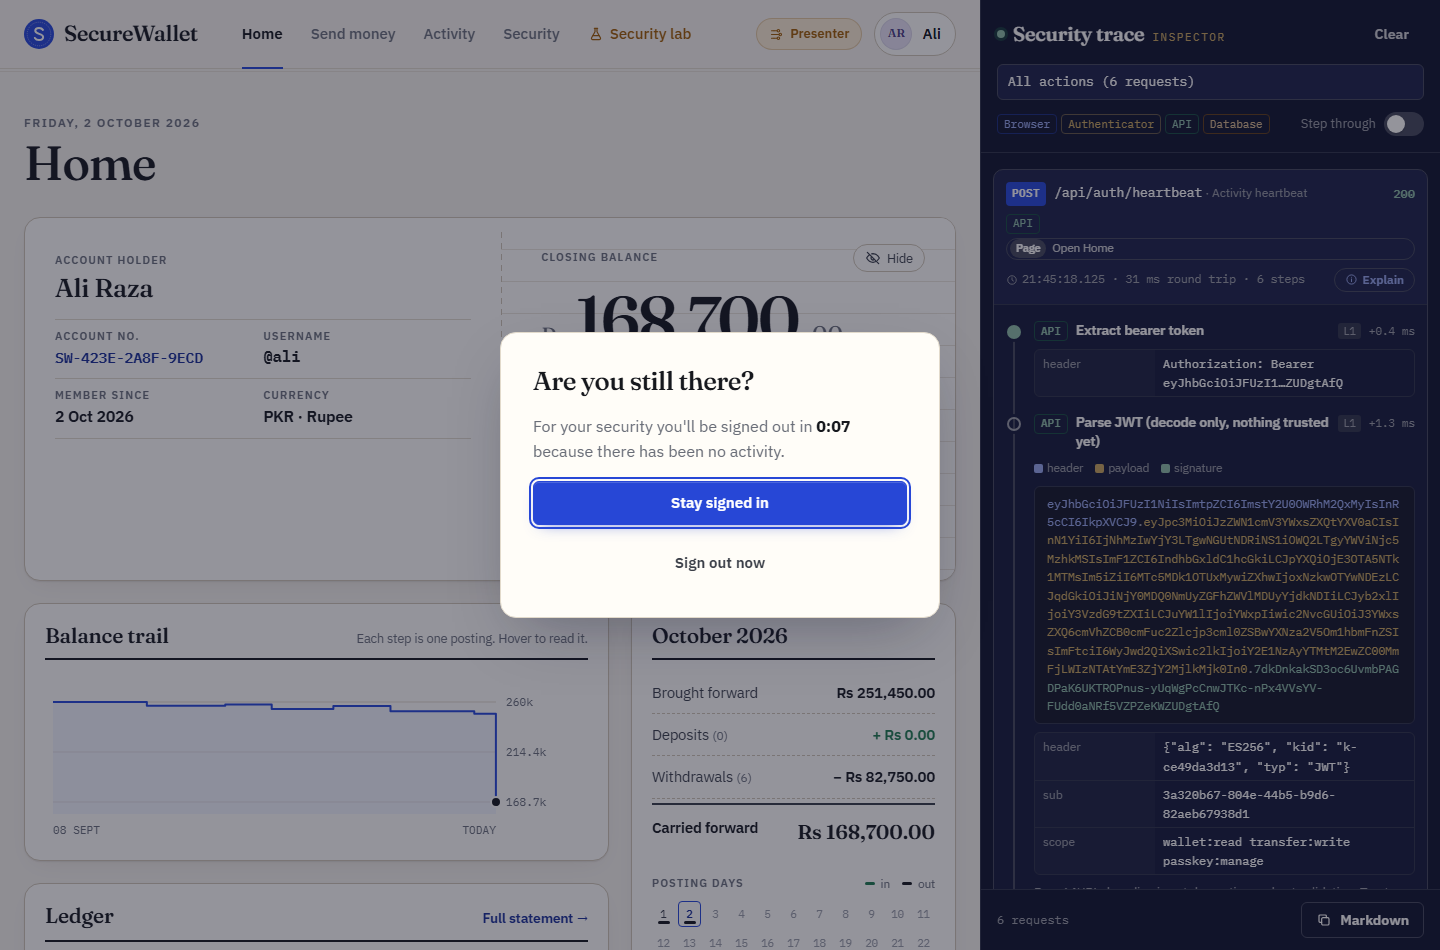
\includegraphics[width=\linewidth]{figures/v2-idle-warning.png}\caption{Warning before the limit (demo limit of 15 seconds).}\end{subfigure}\hfill
\begin{subfigure}{0.49\textwidth}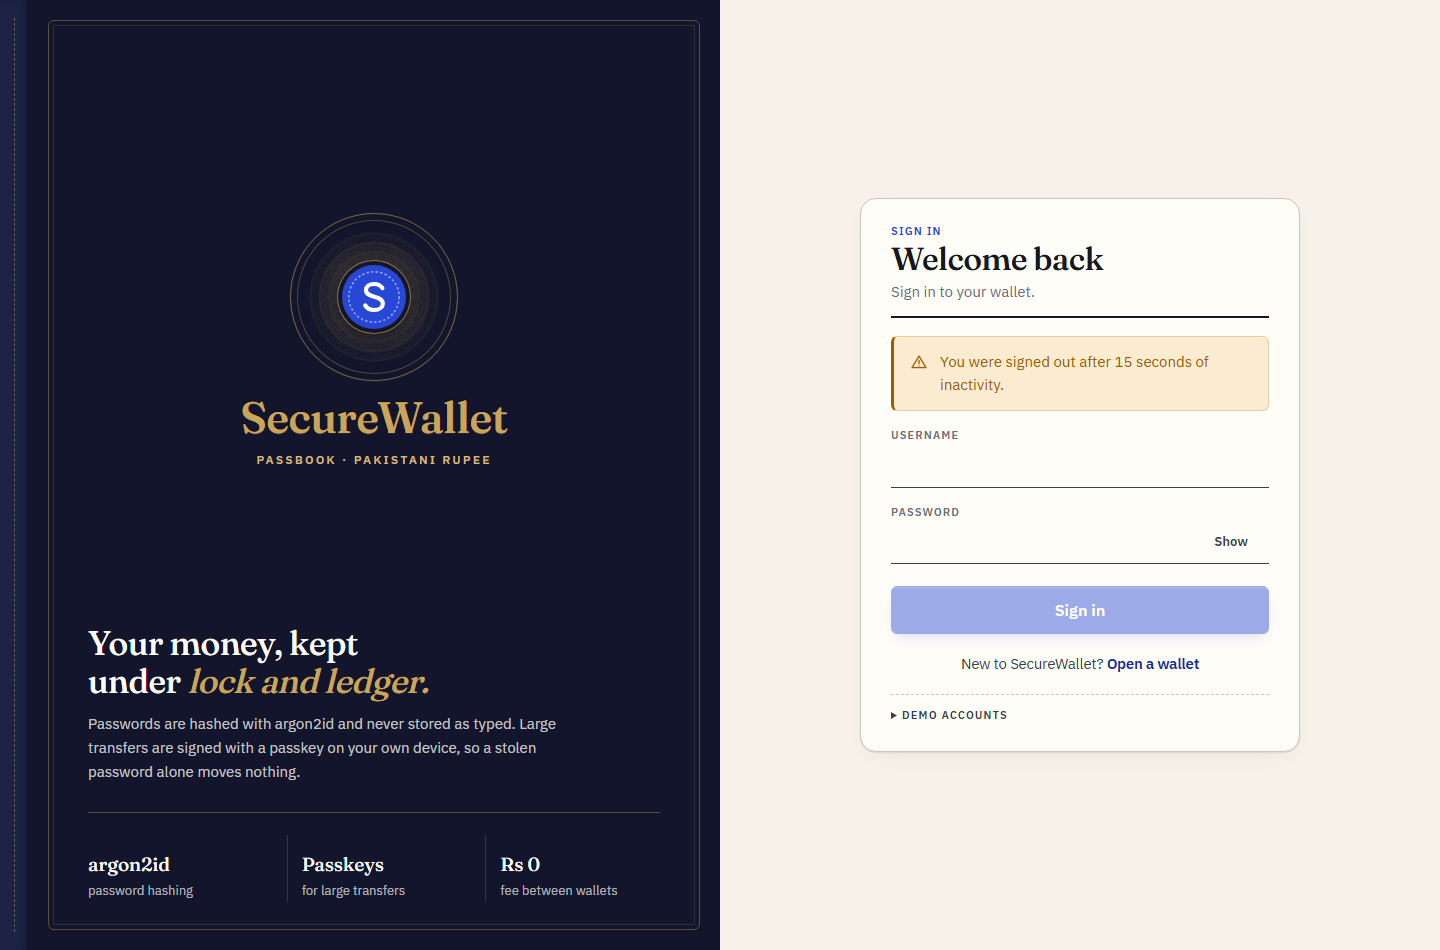
\includegraphics[width=\linewidth]{figures/v2-idle-signed-out.png}\caption{Signed out by the server, with the reason shown.}\end{subfigure}
\caption{W13: the inactivity timeout.}
\label{fig:idle}
\end{figure}

\subsection*{Infrastructure}
\begin{itemize}
\item \textbf{Containers:} they run as non-root with a read-only file system, all Linux capabilities dropped and \code{no-new-privileges}.
\item \textbf{Secrets:} database passwords come from a git-ignored \code{.env}.
\item \textbf{Browser policy:} nginx sends a strict Content-Security-Policy (\code{script-src 'self'}, no third-party origins, fonts self-hosted), \code{X-Frame-Options: DENY}, \code{nosniff} and \code{Referrer-Policy: no-referrer}.
\end{itemize}

\begin{figure}[H]
\centering
\begin{subfigure}{0.40\textwidth}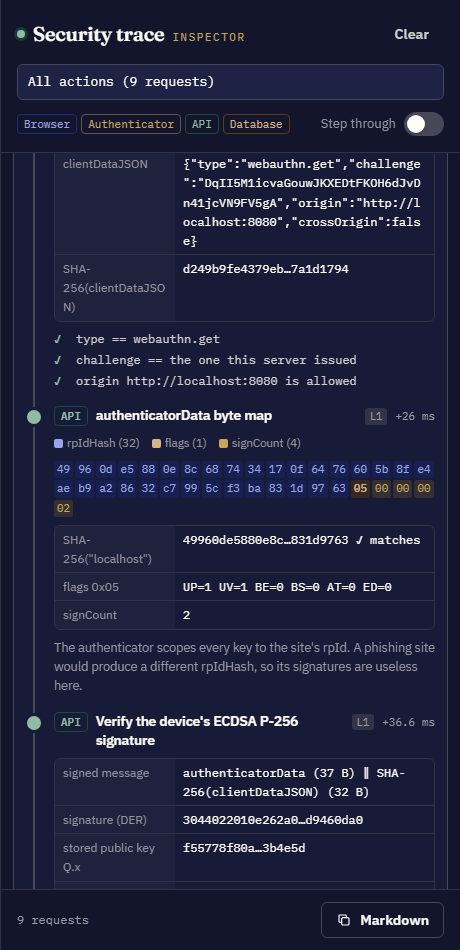
\includegraphics[width=\linewidth]{figures/v2-trace-2.png}\caption{clientDataJSON checks and the authenticatorData byte map (rpIdHash, flags UP=1 UV=1, counter).}\end{subfigure}\hspace{0.05\textwidth}
\begin{subfigure}{0.40\textwidth}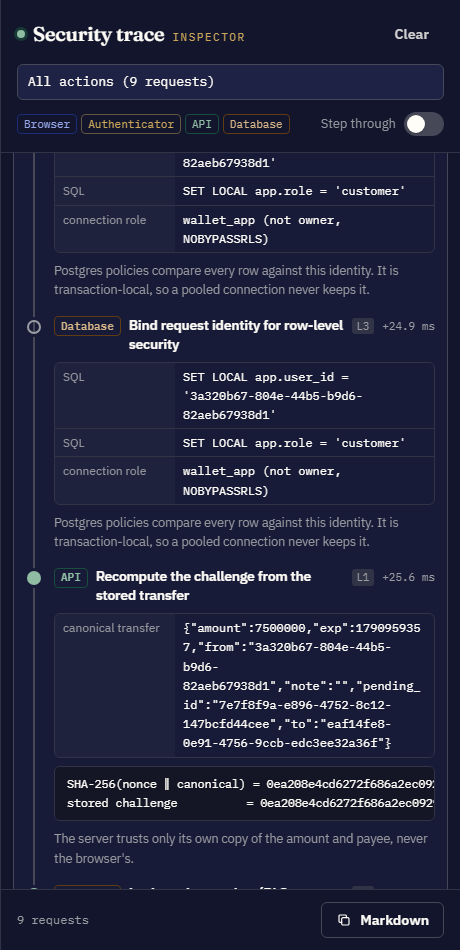
\includegraphics[width=\linewidth]{figures/v2-trace-1.png}\caption{The server recomputes the challenge from its own stored copy of the transfer (SHA-256 of nonce and canonical transfer) and binds the user id for row-level security.}\end{subfigure}
\caption{Security trace of a Rs 75,000 transfer approved with a passkey. Values are from a real run.}
\label{fig:fido2}
\end{figure}

% ------------------------------------------------------------------ 8
\section{Before-and-after security testing}
\label{sec:tests}

\paragraph{Method.} Following the brief's \emph{Weakness $\rightarrow$ Demonstration $\rightarrow$ Control $\rightarrow$ Retest}, each control has a switch in the security lab (demo mode only). For each weakness:
\begin{enumerate}
\item We switch the control off and run the attack: \emph{before}.
\item We switch it on and run the identical attack: \emph{after}.
\end{enumerate}
The switches for W1 and W5 change the real database: they enable or disable the row-level security policies, and drop or re-add the amount constraint. The same pairs are automated in \code{backend/tests/test\_security.py}, which runs against the Docker stack. The final run passed \textbf{\numtests{} of \numtests{} tests} in 5 minutes 27 seconds (19 core security tests, 7 transaction-PIN, 8 encryption-at-rest and 5 session tests).

\begin{table}[H]
\centering\small
\caption{Before/after results (automated tests and live lab).}
\label{tab:results}
\begin{tabularx}{\textwidth}{lP{3.9cm}YY}
\toprule
ID & Attack & Before (control off) & After (control on) \\
\midrule
W1 & Ali requests Sara's wallet by id & \cellcolor{corallight}200: Sara's balance returned & \cellcolor{jadelight}404. With only the API filter off, still 404 because RLS blocks it \\
W2 & Register, then dump the users table & \cellcolor{corallight}\code{plain\$open-sesame-2026} & \cellcolor{jadelight}argon2id hash (\code{\$argon2id\$v=19\$m=65536\ldots}) \\
W3 & 10 wrong passwords, then the right one & \cellcolor{corallight}200: account taken over & \cellcolor{jadelight}429 from the 6th attempt; right password refused while locked \\
W4 & Edit token \code{sub} to Sara, keep signature & \cellcolor{corallight}200: signed in as Sara & \cellcolor{jadelight}401; \code{alg:none} also 401 \\
W5 & Send $-$Rs 5,000 to Sara & \cellcolor{corallight}201: Ali's balance rises by Rs 5,000 & \cellcolor{jadelight}422; also 1.5, \code{"100"}, 0, over-limit, extra \code{balance} field, self-transfer \\
W6 & Same transfer 5 times at once, same key & \cellcolor{corallight}charged more than once & \cellcolor{jadelight}charged once, one reference; changed body gives 409 \\
W7 & 10 parallel Rs 1,000 transfers & \cellcolor{corallight}balance falls by less than recorded; reconciliation fails & \cellcolor{jadelight}exact debit; reconciliation passes \\
W8 & Rs 60,000 with only a session token & \cellcolor{corallight}201: money moved & \cellcolor{jadelight}403 without passkey, 202 with one. Wrong origin 400, tampered challenge 400, replay 409 \\
W9 & Customer reads the audit log & \cellcolor{corallight}200: log exposed & \cellcolor{jadelight}403; reconciliation 403 even with the API check off \\
W10 & Failed login with a wrong password & \multicolumn{2}{P{7cm}}{Always on: the failure is audited with the username and never the password (verified by test).} \\
W11 & Rs 1,000 transfer with only the session, no PIN & \cellcolor{corallight}201: money sent & \cellcolor{jadelight}403 \code{tpin\_required}; 3 wrong PINs give 423 lock \\
W12 & Read a new user's row straight from the database & \cellcolor{corallight}name stored as text: ``Probe Person'' & \cellcolor{jadelight}stored as \code{enc:v1:\ldots} (AES-256-GCM); the app still shows the name \\
W13 & Leave a session idle past the limit, then use its token & \cellcolor{corallight}200: still usable & \cellcolor{jadelight}401 \code{session\_idle}; refresh also refused \\
\bottomrule
\end{tabularx}
\end{table}

The functional tests in the same suite cover:
\begin{itemize}
\item the brief's example (Ali $\rightarrow$ Rs 2,000 $\rightarrow$ Sara): both balances change and both histories show the transaction;
\item an insufficient-funds transfer recorded as \emph{failed};
\item logout revoking the token;
\item registration, including rejection of a duplicate username;
\item refresh-token rotation with reuse detection.
\end{itemize}

\begin{figure}[H]
\centering
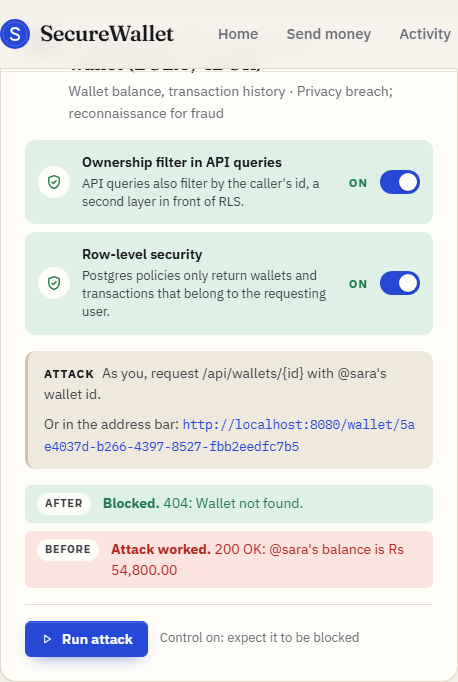
\includegraphics[width=0.5\textwidth]{figures/v2-lab-w1.png}
\caption{Security lab, W1: the \emph{Before} run leaked Sara's balance (red); after both controls were switched back on, the same request was blocked with 404 (green). The trace panel on the right lists the requests, including the rejected \code{GET /api/wallets/\ldots} with status 404.}
\label{fig:lab}
\end{figure}

\begin{figure}[H]
\centering
\begin{subfigure}{0.32\textwidth}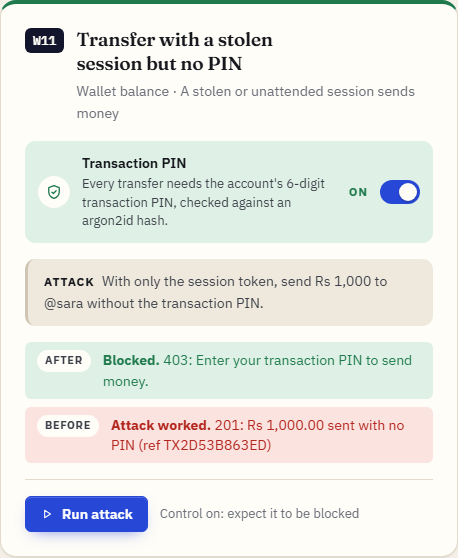
\includegraphics[width=\linewidth]{figures/v2-lab-w11.png}\caption{W11: without the PIN control a session alone sends money (201); with it, 403.}\end{subfigure}\hfill
\begin{subfigure}{0.32\textwidth}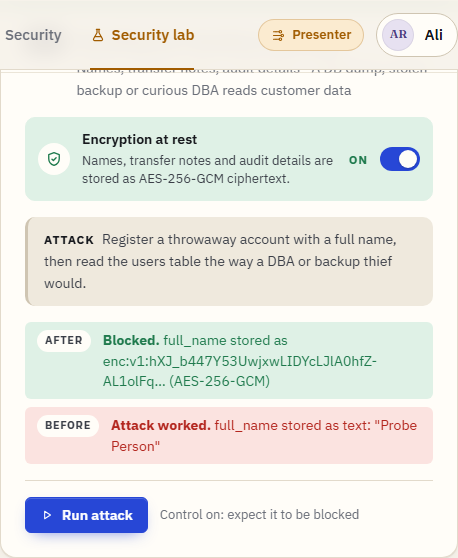
\includegraphics[width=\linewidth]{figures/v2-lab-w12.png}\caption{W12: the stored name is plain text before, \code{enc:v1:\ldots} ciphertext after.}\end{subfigure}\hfill
\begin{subfigure}{0.32\textwidth}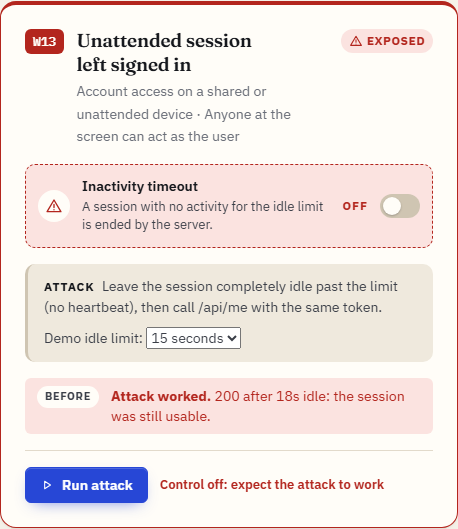
\includegraphics[width=\linewidth]{figures/v2-lab-w13-before.png}\caption{W13 with the control off: the idle session is still usable. With it on, see Figure~\ref{fig:idle}.}\end{subfigure}
\caption{Security lab, before/after runs for the controls added in this iteration.}
\label{fig:lab2}
\end{figure}

\begin{figure}[H]
\centering
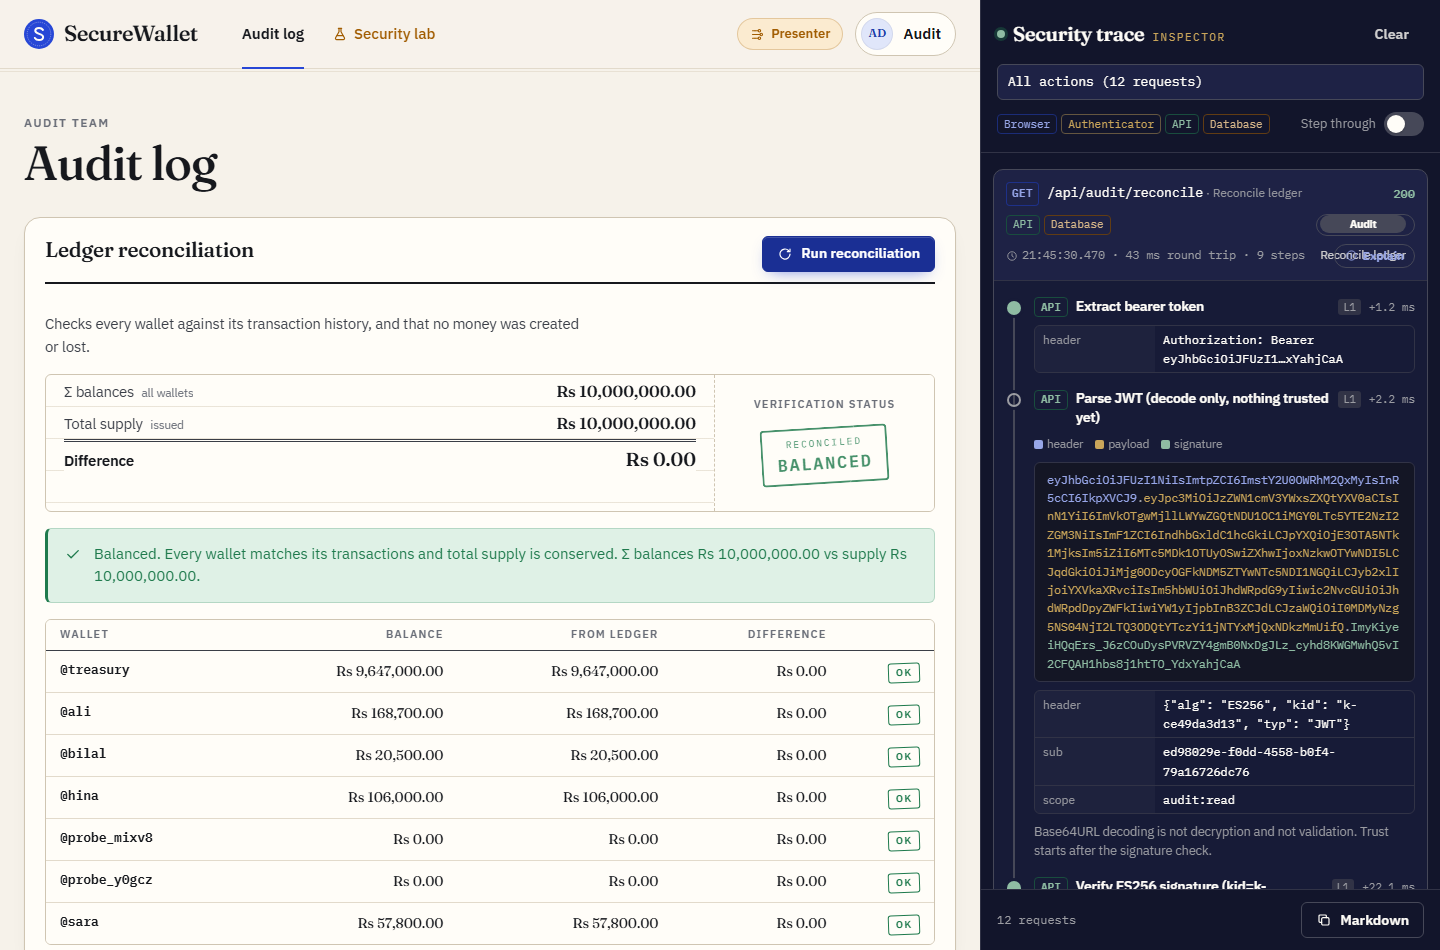
\includegraphics[width=0.85\textwidth]{figures/v2-audit.png}
\caption{Auditor's register: reconciliation stamped BALANCED (every wallet equals its ledger and total supply is conserved), above the append-only audit trail.}
\label{fig:audit}
\end{figure}

% ------------------------------------------------------------------ 9
\begin{landscape}
\section{Security Design Table}
\footnotesize
\setlength{\tabcolsep}{4pt}
\begin{longtable}{P{0.7cm}P{2.6cm}P{3.3cm}P{2.6cm}P{3.4cm}P{5.2cm}P{3.3cm}}
\toprule
ID & Asset / Component & Identified weakness & Possible impact & Proposed control & How the control was implemented & Result \\
\midrule
\endhead
W1 & Wallets, transactions / wallet API and database & BOLA: a changed id in the URL returns another customer's wallet & Privacy breach, fraud reconnaissance & Row-level security plus API ownership filter & RLS policies on \code{wallets} and \code{transactions}; API role \code{wallet\_app} is not owner and has \code{NOBYPASSRLS}; \code{SET LOCAL app.user\_id} per transaction; \code{AND user\_id = :caller} in queries; 404 on mismatch & Before 200 with Sara's data; after 404; RLS alone still blocks \\
\midrule
W2 & Credentials / \code{users} table & Readable password storage & All passwords exposed by one leak & argon2id hashing & \code{passwords.py}: m=64 MiB, t=3, p=2, random 16-byte salt; dummy verify for unknown users; password policy & Stored value changes from plain text to an argon2id hash \\
\midrule
W3 & Login endpoint & Unlimited password guessing & Account takeover & IP rate limit and account lockout & \code{ratelimit.py}: 20 per minute per IP; lockout after 5 failures, 60 s doubling to 15 min; identical error message; nginx outer limit & Before: password found after 10 guesses; after: 429 from the 6th \\
\midrule
W4 & Access token / API & Edited token accepted & Impersonation of any customer & ES256 JWS, full claim validation, revocation & \code{tokens.py}, \code{deps.py}: algorithm pinned, key id, iss/aud/exp/nbf/iat/jti required; revocation list on logout; rotating refresh cookie with reuse detection & Forged token: 200 before, 401 after \\
\midrule
W5 & Balance / transfer API & Invalid amounts and extra fields reach business logic & Money pulled from another wallet & Strict validation in API and database & Pydantic \code{extra="forbid"}, strict integer; Rs 0.01--500,000; re-check in \code{transfer\_funds()}; CHECK constraints & $-$Rs 5,000: 201 before, 422 after \\
\midrule
W6 & Transfer API & Replay and double submit & Customer charged twice & Idempotency keys & \code{Idempotency-Key} header; \code{(user\_id, key)} primary key; stored response replayed; 409 if body differs & 5 identical requests: charged once \\
\midrule
W7 & Balances and ledger / database & Race condition, partial failure & Lost updates, money created or destroyed & Single atomic transfer function with row locks & \code{transfer\_funds()} SECURITY DEFINER; \code{FOR UPDATE} in user-id order; one DB transaction; API role cannot UPDATE balances & 10 parallel: lost updates before; exact and reconciled after \\
\midrule
W8 & High-value transfers & Stolen password or session enough to move large sums & Wallet drained & Risk engine plus FIDO2 step-up bound to the transfer & \code{risk.py}: over Rs 50,000, or new payee over Rs 10,000; 202 pending; challenge = SHA-256(nonce, transfer); origin, rpId, UV, counter and ECDSA signature verified with py\_webauthn & 201 before; 202 then passkey after; phishing origin and replay rejected \\
\midrule
W9 & Audit functions & Customer reaches privileged operations & Exposure and tampering of evidence & Role scopes checked in API and database & Scopes per role in the token; \code{require\_role}; role check inside \code{reconcile\_ledger()} & Customer: 200 before, 403 after; DB still refuses \\
\midrule
W10 & Audit log & Unrecorded rejections, secrets in logs & No accountability, credential leak & Append-only audit log with redaction & \code{audit.py} writes every outcome on its own connection; key-based redaction; UPDATE/DELETE trigger; no stack traces returned & Failed login audited without the password \\
\midrule
W11 & Transfers / transfer API & A live session alone can pay & Hijacked or unattended session drains the wallet & 6-digit transaction PIN on every transfer & \code{tpin.py}, \code{routers/tpin.py}: argon2id hash, weak-PIN list, 3 tries then 15-minute lock, checked first in \code{create\_transfer} & No PIN: 201 before, 403 after \\
\midrule
W12 & Names, notes, audit details / database & Stored as readable text & Dump or backup exposes customer data & AES-256-GCM encryption at rest & \code{crypto.py}: \code{enc:v1} format, per-row AAD, key in the keys volume; encrypt on write, decrypt on read & DB shows ciphertext; app shows plaintext \\
\midrule
W13 & Sessions / API & Session never ends while the tab is open & Unattended screen used by someone else & Server-enforced idle timeout & \code{sessions.py}: \code{sessions} table, \code{sid} claim, idle and absolute limits checked on every request and on refresh; heartbeat and warning in the browser & Idle token: 200 before, 401 after \\
\bottomrule
\end{longtable}
\end{landscape}

% ------------------------------------------------------------------ 10
\section{Security principles applied}

\begin{table}[H]
\centering\small
\caption{How the design relates to the Unit 1 principles (brief \S8).}
\begin{tabularx}{\textwidth}{P{3.6cm}Y}
\toprule
Principle & Where it is applied \\
\midrule
Confidentiality & RLS and ownership checks (W1); argon2id (W2); encryption at rest (W12); lookups return only name and username, never ids or balances. \\
Integrity & Signed tokens (W4); validation in three places (W5); idempotency (W6); atomic transfers with locks (W7); transfer-bound passkey approval (W8). \\
Availability & Rate limits protect the login and the API; the database refuses to start a transfer it cannot finish; the stack restarts automatically. \\
Authentication & argon2id passwords, lockout, ES256 tokens, the transaction PIN on every transfer (W11), the inactivity timeout (W13), passkeys for high-risk actions. \\
Authorization & Scopes per role, object ownership in the API and the database. \\
Least privilege & The API's database role cannot update balances or insert transactions directly; auditors cannot move money; customers cannot audit. \\
Secure defaults & Demo mode is off by default, so the lab and trace do not exist; every lab switch starts in the secure position. \\
Separation of responsibilities & Customer and auditor roles; the database owner role is used only for migrations. \\
Defence in depth & payments need a session, then the PIN (W11), then a passkey above the limit (W8); W1 (API filter and RLS), W5 (schema, API rules, DB function, constraints), W9 (API and database role checks). \\
Reduction of unnecessary exposure & The database has no published port; responses carry minimal fields; errors carry no internal details. \\
Logging and accountability & Append-only audit log of every outcome, with secrets redacted (W10). \\
Resilience & Atomic transactions leave no partial state; idempotent retries are safe; reconciliation detects inconsistencies. \\
\bottomrule
\end{tabularx}
\end{table}

% ------------------------------------------------------------------ 11
\section{Individual student contributions}

\begin{table}[H]
\centering\small
\caption{Contributions of each group member.}
\begin{tabularx}{\textwidth}{P{4cm}Y}
\toprule
Student & Major contribution \\
\midrule
Israr Ahmed (26I-7722) & Architecture and Docker setup; database schema, row-level security and the atomic transfer function (W1, W7); authentication: password hashing, throttling, signed tokens and refresh sessions (W2--W4); encryption at rest (W12); audit log (W10); security lab and the automated before/after tests. \\
Burhan Ud Din (26I-7711) & Transfers, server-side validation and idempotency (W5, W6); passkeys and the risk engine (W8); roles and the auditor desk (W9); transaction PIN (W11); inactivity timeout (W13); the passbook front end and security trace; security analysis and this report. \\
\bottomrule
\end{tabularx}
\end{table}

Every member can explain the whole application, as the brief requires.

% ------------------------------------------------------------------ 12
\section{Limitations and future improvements}

\begin{itemize}
\item \textbf{No TLS in the local stack.} Traffic between the browser and nginx is plain HTTP, which WebAuthn allows only on \code{localhost}. A deployment would terminate TLS 1.3 at nginx.
\item \textbf{Keys in a Docker volume.} The token signing key sits in a Docker volume. Production would keep it in a key-management service or HSM and rotate it using the existing key id.
\item \textbf{In-memory rate limiter.} The per-IP limiter lives in the API process. Several API instances would need a shared store such as Redis. The per-account lockout is already in the database.
\item \textbf{No real funding source.} Money enters only through seeded treasury deposits. A top-up from a bank would need a signed, replay-protected payment callback (Lecture 1, slide 19).
\item \textbf{Simple risk engine.} It uses amount and payee history only. Velocity limits, device recognition and new-login alerts are natural next steps.
\item \textbf{Stolen session cookie: analysed, not demonstrated.} The refresh token sits in an \code{HttpOnly; SameSite=Strict} cookie, so page scripts cannot read it and other sites cannot send it; it is rotated on every use, with reuse detection that revokes the whole session; and the idle timeout (W13) limits how long a copy stays useful. A copied cookie replayed directly, however, would still be accepted until one of those triggers. The planned fix, binding the session to a non-extractable key held by the browser (DPoP-style device binding), and a lab demonstration of the replay were not built in this iteration.
\item \textbf{Encryption key and balances.} The data key lives in the Docker keys volume; production would use a KMS or HSM with envelope encryption. Balances and usernames are not encrypted, by design (Section 7, W12).
\item \textbf{PIN space.} A 6-digit PIN has one million values. Online guessing is stopped by the 3-try lock, but if the database and the hashes were stolen, argon2id only slows an offline search; it cannot make one million guesses infeasible.
\item \textbf{Lab reset clears the audit log.} This is an intentional demo-only owner action. It does not exist when demo mode is off.
\end{itemize}

\appendix
\section{Running the system}
\begin{lstlisting}
cp .env.example .env          # set the three database passwords
docker compose up --build     # open http://localhost:8080
# demo accounts: ali, sara, bilal, hina, auditor  (password Wallet@2026!)

# tests (API exposed on 127.0.0.1:8000)
docker compose -f docker-compose.yml -f docker-compose.dev.yml up -d --build
pytest backend/tests -v
\end{lstlisting}

\section{Security trace (presenter mode)}
When presenter mode is on, the front end sends the header \code{X-Security-Trace: 1}. The backend records each security decision it makes for that request and returns the steps with the response. Examples: the token signature check with its ECDSA arithmetic, the claims, the RLS identity binding, validation rules, the risk decision, the SQL of the transfer, and the audit record.

The panel adds several aids for the demonstration:
\begin{itemize}
\item It groups requests by the user action that caused them, and a filter shows a single action (Figure~\ref{fig:trace}).
\item Each request is tagged with the components it touched and the time it was sent.
\item An \emph{Explain} button describes each request in plain language.
\end{itemize}
Without demo mode the header is ignored and nothing is collected.

\begin{figure}[H]
\centering
\begin{subfigure}{0.62\textwidth}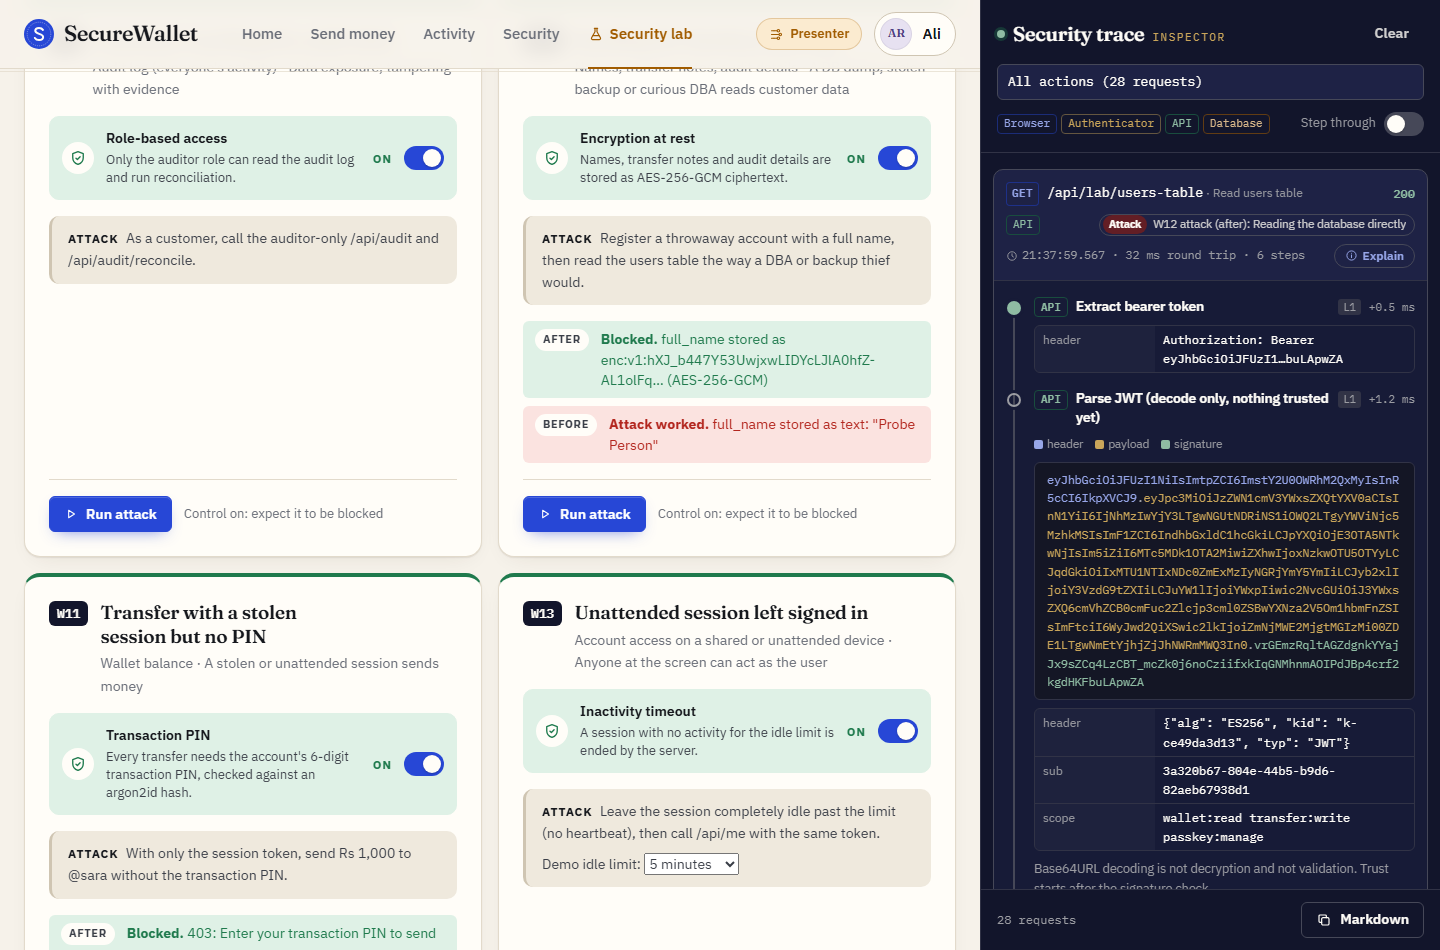
\includegraphics[width=\linewidth]{figures/v2-lab-page.png}\caption{Security lab with the trace panel: each request is tagged with the action that caused it (here the W12 attack), the time it was sent and the parts of the system it touched.}\end{subfigure}
\caption{The security trace used during the live demonstration.}
\label{fig:trace}
\end{figure}

\end{document}
